\iffalse
\documentclass[journal,12pt,twocolumn]{IEEEtran}
\usepackage{setspace}
\usepackage{gensymb}
\usepackage{xcolor}
\usepackage{caption}
\singlespacing
\usepackage{siunitx}
\usepackage[cmex10]{amsmath}
\usepackage{mathtools}
\usepackage{hyperref}
\usepackage{amsthm}
\usepackage{mathrsfs}
\usepackage{txfonts}
\usepackage{stfloats}
\usepackage{cite}
\usepackage{cases}
\usepackage{subfig}
\usepackage{longtable}
\usepackage{multirow}
\usepackage{enumitem}
\usepackage{bm}
\usepackage{mathtools}
\usepackage{listings}
\usepackage{tikz}
\usetikzlibrary{shapes,arrows,positioning}
\usepackage{circuitikz}
\renewcommand{\vec}[1]{\boldsymbol{\mathbf{#1}}}
\DeclareMathOperator*{\Res}{Res}
\renewcommand\thesection{\arabic{section}}
\renewcommand\thesubsection{\thesection.\arabic{subsection}}
\renewcommand\thesubsubsection{\thesubsection.\arabic{subsubsection}}

\renewcommand\thesectiondis{\arabic{section}}
\renewcommand\thesubsectiondis{\thesectiondis.\arabic{subsection}}
\renewcommand\thesubsubsectiondis{\thesubsectiondis.\arabic{subsubsection}}
\hyphenation{op-tical net-works semi-conduc-tor}

\lstset{
language=Python,
frame=single, 
breaklines=true,
columns=fullflexible
}
\begin{document}
\theoremstyle{definition}
\newtheorem{theorem}{Theorem}[section]
\newtheorem{problem}{Problem}
\newtheorem{proposition}{Proposition}[section]
\newtheorem{lemma}{Lemma}
\newtheorem{corollary}[theorem]{Corollary}
\newtheorem{example}{Example}[section]
\newtheorem{definition}{Definition}[section]
\newcommand{\BEQA}{\begin{eqnarray}}
\newcommand{\EEQA}{\end{eqnarray}}
\newcommand{\define}{\stackrel{\triangle}{=}}
\newcommand{\myvec}[1]{\ensuremath{\begin{pmatrix}#1\end{pmatrix}}}
\newcommand{\mydet}[1]{\ensuremath{\begin{vmatrix}#1\end{vmatrix}}}
\bibliographystyle{IEEEtran}
\providecommand{\nCr}[2]{\,^{#1}C_{#2}} % nCr
\providecommand{\nPr}[2]{\,^{#1}P_{#2}} % nPr
\providecommand{\mbf}{\mathbf}
\providecommand{\pr}[1]{\ensuremath{\Pr\left(#1\right)}}
\providecommand{\qfunc}[1]{\ensuremath{Q\left(#1\right)}}
\providecommand{\sbrak}[1]{\ensuremath{{}\left[#1\right]}}
\providecommand{\lsbrak}[1]{\ensuremath{{}\left[#1\right.}}
\providecommand{\rsbrak}[1]{\ensuremath{{}\left.#1\right]}}
\providecommand{\brak}[1]{\ensuremath{\left(#1\right)}}
\providecommand{\lbrak}[1]{\ensuremath{\left(#1\right.}}
\providecommand{\rbrak}[1]{\ensuremath{\left.#1\right)}}
\providecommand{\cbrak}[1]{\ensuremath{\left\{#1\right\}}}
\providecommand{\lcbrak}[1]{\ensuremath{\left\{#1\right.}}
\providecommand{\rcbrak}[1]{\ensuremath{\left.#1\right\}}}
\theoremstyle{remark}
\newtheorem{rem}{Remark}
\newcommand{\sgn}{\mathop{\mathrm{sgn}}}
\newcommand{\rect}{\mathop{\mathrm{rect}}}
\newcommand{\sinc}{\mathop{\mathrm{sinc}}}
\providecommand{\abs}[1]{\left\vert#1\right\vert}
\providecommand{\res}[1]{\Res\displaylimits_{#1}} 
\providecommand{\norm}[1]{\left\Vert#1\right\Vert}
\providecommand{\mtx}[1]{\mathbf{#1}}
\providecommand{\mean}[1]{E\left[ #1 \right]}
\providecommand{\fourier}{\overset{\mathcal{F}}{ \rightleftharpoons}}
\providecommand{\ztrans}{\overset{\mathcal{Z}}{ \rightleftharpoons}}
\providecommand{\system}[1]{\overset{\mathcal{#1}}{ \longleftrightarrow}}
\newcommand{\solution}{\noindent \textbf{Solution: }}
\providecommand{\dec}[2]{\ensuremath{\overset{#1}{\underset{#2}{\gtrless}}}}
\let\StandardTheFigure\thefigure
\def\putbox#1#2#3{\makebox[0in][l]{\makebox[#1][l]{}\raisebox{\baselineskip}[0in][0in]{\raisebox{#2}[0in][0in]{#3}}}}
     \def\rightbox#1{\makebox[0in][r]{#1}}
     \def\centbox#1{\makebox[0in]{#1}}
     \def\topbox#1{\raisebox{-\baselineskip}[0in][0in]{#1}}
     \def\midbox#1{\raisebox{-0.5\baselineskip}[0in][0in]{#1}}

\vspace{3cm}
\title{Circle Assignment}
\author{Gautam Singh}
\maketitle
\bigskip

\begin{abstract}
    This document contains the solution to Question 13 of 
    Exercise 2 in Chapter 10 of the class 10 NCERT textbook.
\end{abstract}

\begin{enumerate}
       \solution 
\fi
		We begin by proving a useful lemma.
    \begin{lemma}
        The line joining the centre of the circle to an external point bisects
        the angle subtended by the tangent chord at the centre.
    \end{lemma}
    \begin{proof}
        Refer to Fig. \ref{fig:chapters/10/10/2/13/tangent}.
 Set $\vec{O}$ to be the origin. Since 
        $OA \perp AP$,
        \begin{align}
            \vec{A}^\top\brak{\vec{A}-\vec{P}} &= 0 \\
            \implies \vec{A}^\top\vec{P} &= \norm{\vec{A}}^2
            \label{eq:chapters/10/10/2/13/a-p}
        \end{align}
        Similarly,
        \begin{align}
            \vec{B}^\top\vec{P} = \norm{\vec{B}}^2
            \label{eq:chapters/10/10/2/13/b-p}
        \end{align}
        Since $\vec{A}$ and $\vec{B}$ lie on the circle, their norms are equal.
        Thus, from \eqref{eq:chapters/10/10/2/13/a-p} and \eqref{eq:chapters/10/10/2/13/b-p},
        \begin{align}
            \vec{A}^\top\vec{P} = \vec{B}^\top\vec{P}
        \end{align}
        and the lemma follows.
        \begin{figure}[!ht]
            \centering
            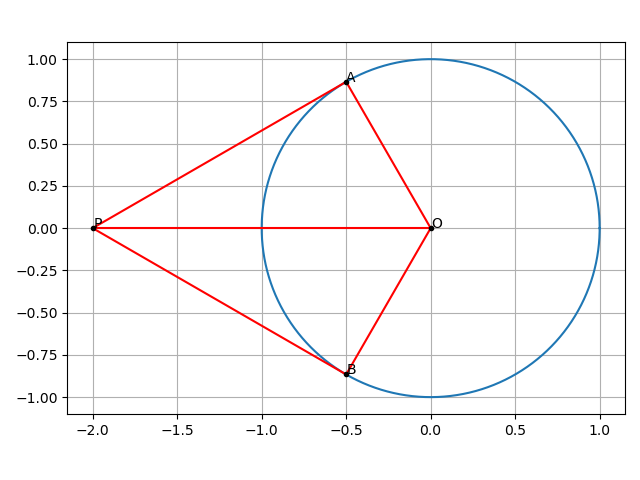
\includegraphics[width=\columnwidth]{chapters/10/10/2/13/figs/tangent.png}
            \caption{$OP$ bisects $\angle AOB$.}
            \label{fig:chapters/10/10/2/13/tangent}
        \end{figure}
    \end{proof}
    Call the quadrilateral $ABCD$, where
    \begin{align}
        \vec{A} = \myvec{-2\\0},\ \vec{C} = \myvec{1\\1}
        \label{eq:chapters/10/10/2/13/a-c-def}
    \end{align}
    Suppose that $ABCD$ circumscribes the unit circle, given by
    \begin{align}
        \vec{x}^\top\vec{x} - 1 = 0
        \label{eq:chapters/10/10/2/13/unit-circ}
    \end{align}
    Comparing \eqref{eq:chapters/10/10/2/13/unit-circ} with the general equation of the circle,
    \begin{align}
        \vec{u} = \vec{0},\ f = -1
        \label{eq:chapters/10/10/2/13/u-f-val}
    \end{align}
    To find the points of contact from $\vec{A}$, we have
    \begin{align}
        \vec{\Sigma_A} &= \brak{\vec{A}+\vec{u}}\brak{\vec{A}+\vec{u}}^\top - \brak{\vec{A}^\top\vec{A}+2\vec{u}^\top\vec{A} + f}\vec{I} \\
                     &= \myvec{1&0\\0&-3}
                     \label{eq:chapters/10/10/2/13/sigma}
    \end{align}
    The eigenvalues of $\vec{\Sigma_A}$ are
    \begin{align}
        \lambda_1 = 1,\ \lambda_2 = -3
        \label{eq:chapters/10/10/2/13/lambda}
    \end{align}
    and since the eigenvector matrix $\vec{P_A} = \vec{I}$,
    \begin{align}
        \vec{n_1} = \myvec{1\\\sqrt{3}},\ \vec{n_2} = \myvec{1\\-\sqrt{3}}
        \label{eq:chapters/10/10/2/13/n-sigma}
    \end{align}
    Thus, the points of contact are given by
    \begin{align}
        \vec{E} = \frac{1}{2}\myvec{-1\\\sqrt{3}},\ \vec{H} = \frac{1}{2}\myvec{-1\\-\sqrt{3}}
        \label{eq:chapters/10/10/2/13/poc-eh}
    \end{align}
    Similarly for $\vec{C}$,
    \begin{align}
        \vec{\Sigma_C} = \myvec{1&1\\1&1} - \vec{I} = \myvec{0&1\\1&0}
    \end{align}
    Notice that
    \begin{align}
        \vec{\Sigma_C}\myvec{1\\1} &= \myvec{1\\1} \\
        \vec{\Sigma_C}\myvec{1\\-1} &= -\myvec{1\\-1} \\
    \end{align}
    Thus, the eigenvalues and the corresponding eigenvector
    matrix is
    \begin{align}
        \mu_1 = 1,\ \mu_2 = -1,\ \vec{P_C} = \myvec{1&1\\1&-1}
    \end{align}
    and thus
    \begin{align}
        \vec{m_1} &= \vec{P_C}\myvec{1\\1} = \myvec{2\\0} \\ 
        \vec{m_2} &= \vec{P_C}\myvec{1\\-1} = \myvec{0\\2}
    \end{align}
    Therefore, the points of contact of $\vec{C}$ are
    \begin{align}
        \vec{F} = \myvec{1\\0},\ \vec{G} = \myvec{0\\1}
        \label{eq:chapters/10/10/2/13/poc-fg}
    \end{align}
    Using the lemma we proved above, the direction vectors of $\vec{B}$ and 
    $\vec{D}$ are
    \begin{align}
        \vec{d_B} &= \vec{E} + \vec{F} = \frac{\sqrt{3}}{2}\myvec{\sqrt{3}\\1} \label{eq:chapters/10/10/2/13/d-B} \\
        \vec{d_D} &= \vec{G} + \vec{H} = \frac{1}{2}\myvec{-1\\2-\sqrt{3}} \label{eq:chapters/10/10/2/13/d-D}
    \end{align}
    Clearly,
    \begin{align}
        \norm{\vec{d_B}} &= \sqrt{3} \\
        \norm{\vec{d_D}} &= \sqrt{2-\sqrt{3}}
        \label{eq:chapters/10/10/2/13/norm-d}
    \end{align}
    and from \eqref{eq:chapters/10/10/2/13/a-c-def}, \eqref{eq:chapters/10/10/2/13/d-B} and \eqref{eq:chapters/10/10/2/13/d-D},
    \begin{align}
        \cos\angle AOD &= \frac{\vec{A}^\top\vec{d_D}}{\norm{A}\norm{\vec{d_D}}} \\
                       &= \frac{-1}{2\sqrt{2\sqrt{3}}} \\
                       &= -\frac{\sqrt{2+\sqrt{3}}}{2} \\
                       &= -\frac{\sqrt{3}+1}{2\sqrt{2}} \label{eq:chapters/10/10/2/13/cos-aod} \\
        \cos\angle BOC &= \frac{\vec{C}^\top\vec{d_B}}{\norm{C}\norm{\vec{d_B}}} \\
                       &= \frac{\sqrt{3}+1}{2\sqrt{2}} \label{eq:chapters/10/10/2/13/cos-boc}
    \end{align}
    Hence, from \eqref{eq:chapters/10/10/2/13/norm-d}, \eqref{eq:chapters/10/10/2/13/cos-aod} and \eqref{eq:chapters/10/10/2/13/cos-boc},
    \begin{align}
        \cos\angle AOD + \cos\angle BOC = 0
    \end{align}
    and hence, $\angle AOD + \angle BOC = \pi$, as required.

    The situation is illustrated in Fig. \ref{fig:chapters/10/10/2/13/quad-circ}. The numerical parameters used 
    in the construction are shown in Table \ref{tab:chapters/10/10/2/13/param}.
    \begin{table}[!ht]
        \centering
        \begin{tabular}{|c|c|}
            \hline
            \textbf{Parameter} & \textbf{Value} \\
            \hline
            $r$ & 1 \\
            \hline
            $\vec{A}$ & $\myvec{-2\\0}$ \\
            \hline
            $\vec{C}$ & $\myvec{1\\1}$ \\
            \hline
        \end{tabular}
        \caption{Parameters used in the construction of Fig. \ref{fig:chapters/10/10/2/13/quad-circ}.}
        \label{tab:chapters/10/10/2/13/param}
    \end{table}
    \begin{figure}[!ht]
        \centering
        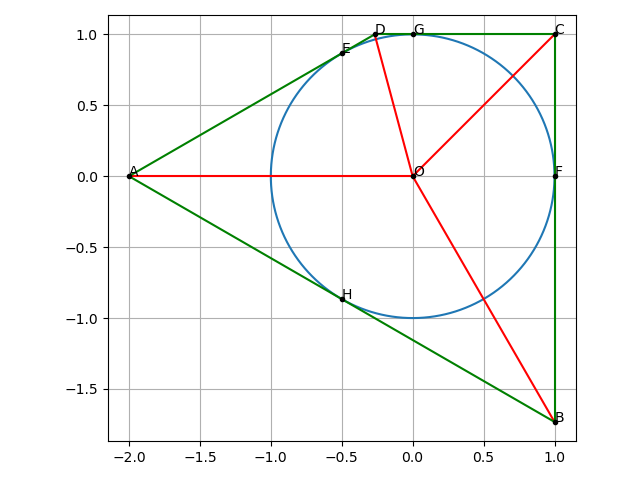
\includegraphics[width=\columnwidth]{chapters/10/10/2/13/figs/quad_circ.png}
        \caption{Angles subtended by the opposite sides of a circumscribing quadrilateral at the center of its incircle are supplementary.}
        \label{fig:chapters/10/10/2/13/quad-circ}
    \end{figure}
